%% 
%% Copyright 2007-2020 Elsevier Ltd
%% 
%% This file is part of the 'Elsarticle Bundle'.
%% ---------------------------------------------
%% 
%% It may be distributed under the conditions of the LaTeX Project Public
%% License, either version 1.2 of this license or (at your option) any
%% later version.  The latest version of this license is in
%%    http://www.latex-project.org/lppl.txt
%% and version 1.2 or later is part of all distributions of LaTeX
%% version 1999/12/01 or later.
%% 
%% The list of all files belonging to the 'Elsarticle Bundle' is
%% given in the file `manifest.txt'.
%% 

%% Template article for Elsevier's document class `elsarticle'
%% with numbered style bibliographic references
%% SP 2008/03/01
%%
%% 
%%
%% $Id: elsarticle-template-num.tex 190 2020-11-23 11:12:32Z rishi $
%%
%%
% \documentclass[5p,times]{elsarticle}

%% Use the option review to obtain double line spacing
%% \documentclass[authoryear,preprint,review,12pt]{elsarticle}

%% Use the options 1p,twocolumn; 3p; 3p,twocolumn; 5p; or 5p,twocolumn
%% for a journal layout:
%% \documentclass[final,1p,times]{elsarticle}
%% \documentclass[final,1p,times,twocolumn]{elsarticle}
%% \documentclass[final,3p,times]{elsarticle}
%% \documentclass[final,3p,times,twocolumn]{elsarticle}
\documentclass[final,5p,times]{elsarticle}
% \documentclass[final,5p,times,twocolumn]{elsarticle}

%% For including figures, graphicx.sty has been loaded in
%% elsarticle.cls. If you prefer to use the old commands
%% please give \usepackage{epsfig}
% \usepackage{epsfig}

%% The amssymb package provides various useful mathematical symbols
\usepackage{amssymb}
\usepackage{algorithm,algorithmic}
\usepackage{multirow}
%% The amsthm package provides extended theorem environments
\usepackage{amsthm}
\usepackage{amsmath}
\usepackage{booktabs} %三线表
\usepackage{graphicx} %图片
\usepackage{stfloats}
\usepackage{array}
\usepackage[T1]{fontenc} % 保证英文字体加粗有效

%% The lineno packages adds line numbers. Start line numbering with
%% \begin{linenumbers}, end it with \end{linenumbers}. Or switch it on
%% for the whole article with \linenumbers.
% \usepackage{lineno}

\journal{Future Generation Computer Systems}

\begin{document}

\begin{frontmatter}

%% Title, authors and addresses

% use the tnoteref command within \title for footnotes;
% use the tnotetext command for theassociated footnote;
% use the fnref command within \author or \address for footnotes;
% use the fntext command for theassociated footnote;
% use the corref command within \author for corresponding author footnotes;
% use the cortext command for theassociated footnote;
% use the ead command for the email address,
% and the form \ead[url] for the home page:
% \title{Title\tnoteref{[a]}}
% \tnotetext[a]{}

% \author[1]{Yapeng Zhi\fnref{fn2}}
\author[1]{Yapeng Zhi}
\ead{1024041011@njupt.edu.cn}
\affiliation[1]{organization={Jiangsu Key Laboratory of Big Data Security and Intelligent Processing},%Department and Organization
            addressline={School of Computer Science, Nanjing University of Posts and Telecommunications}, 
            city={Nanjing},
            postcode={210023}, 
            country={China}}

\author[2]{Xiaolong Xu\corref{cor1}}
\ead{xuxl@njupt.edu.cn}
\cortext[cor1]{Corresponding author. Tel.: +86–13813885172}

\affiliation[2]{organization={School of Computer Science, Nanjing University of Posts and Telecommunications},
            city={Nanjing},
            postcode={210023},
            country={China}}

\title{GHT: Generalizable Hybrid Training for Robust Deepfake Detection}

%% use optional labels to link authors explicitly to addresses:
%% \author[label1,label2]{}
%% \affiliation[label1]{organization={},
%%             addressline={},
%%             city={},
%%             postcode={},
%%             state={},
%%             country={}}
%%
%% \affiliation[label2]{organization={},
%%             addressline={},
%%             city={},
%%             postcode={},
%%             state={},
%%             country={}}

\begin{abstract}
To address the critical issues of poor cross-dataset generalization and insufficient robustness to unknown forgery techniques in deepfake detection, we propose a novel Generalized Hybrid Training (GHT) framework. The framework adopts a generalizable hybrid training strategy that integrates deepfake data and blendfake forgeries to enhance the model's generalizability across various manipulation techniques and datasets. Specifically, we employ Dinov2-small as the backbone network to fully leverage its powerful feature representation capabilities. To effectively integrate multi-scale visual information, we propose an Adaptive Token Mixing (ATM) mechanism capable of dynamically integrating features across multiple levels of the spatial hierarchy. In addition, we propose a Latent Space Contrastive Regularization (LSCR) method to address the common issue of a disorganized latent space arising from hybrid training. By adjusting the distances between positive and negative pairs in the latent space, this method enhances feature discriminability and mitigates overfitting. Extensive experiments conducted on four benchmark datasets: Celeb-DFv1, Celeb-DFv2, DFDCP, and DFDC demonstrate that, compared to state-of-the-art methods on the DeepfakeBench platform, GHT achieves an average AUC improvement of 5.62\% in cross-domain detection scenarios. Ablation studies and t-SNE visualization analyses further validate the significant roles of hybrid training and latent space regularization in improving the model's generalization capability. These results indicate that GHT holds great potential for developing more robust and adaptable deepfake detection systems.

\end{abstract}

%%Graphical abstract
\begin{graphicalabstract}
\centering
\includegraphics[width=2.0\linewidth]{images/Fig3.pdf}
\end{graphicalabstract}

%%Research highlights
\begin{highlights}
\item Lightweight Dinov2-based model achieves high performance with low computational cost.
\item Blendfakes used as augmentation to ease feature disorganization in hybrid training.
\item GHT framework applies blendfakes for latent regularization, improving generalization.
\end{highlights}

\begin{keyword}
Deepfake Detection \sep 
Hybrid Training \sep 
Latent Space Regularization  \sep 
Generalization
\end{keyword}

\end{frontmatter}

%% \linenumbers
%% main text

\section{Introduction}

Deepfake is a synthetic media technology based on artificial intelligence which, in a narrower sense, refers to the manipulation and replacement of human faces using deep learning algorithms. Compared with other forgery techniques, facial deepfakes are particularly deceptive, as they can generate highly realistic facial images or videos that are difficult for the public to distinguish from real content. In recent years, misuse of this technology has posed serious threats to social security, political stability, and personal privacy, especially in domains such as financial fraud, public opinion manipulation, and identity theft. Since the face is a key feature of identity recognition, its forgery can more easily trigger trust crises and exacerbate information pollution. Therefore, it is imperative to develop precise and efficient detection methods to identify and filter facial forgery content, maintaining the credibility and health of the information ecosystem.

However, facial deepfake detection presents significant challenges and differs from conventional image classification tasks. Forgery techniques are evolving rapidly, with increasingly diverse generation methods, making it difficult for detection models to generalize to unknown forgery types. Moreover, deepfake faces typically maintain a high level of overall realism, with only subtle alterations in localized regions. This causes models to overfit specific datasets and perform poorly when encountering unseen datasets or forgery methods \cite{1}. Hence, improving the generalizability of detection models so that they remain robust under different forgery techniques and diverse data distributions is a core issue in deepfake detection research.

Currently, significant progress has been made in deepfake detection technologies, which can be divided into feature engineering based methods and end-to-end methods. Feature engineering methods rely on manually extracting specific attributes of genuine faces such as depth of field \cite{2}, color components \cite{3}, head pose \cite{4}, lip movement \cite{5}, and biosignals \cite{6,7} to capture and distinguish forgery traces. With the rapid advancement of deep learning, end-to-end methods have gradually demonstrated superior detection performance. These methods learn forgery patterns directly from the data, enabling automatic detection in more complex environments. In end-to-end detection methods, forgery region localization \cite{8} identifies tampered regions with finer granularity; capsule networks \cite{9} preserve spatial relationships between features through their specialized network structures, enabling better characterization of manipulation artifacts; disentangled learning \cite{10,11} decomposes various properties of fake images (such as texture and color) into independent subspaces to more clearly analyze forgery patterns; image reconstruction \cite{12} identifies forgery traces by comparing reconstruction errors between original and forged images; and erasure-based techniques \cite{13} simulate region erasure operations during the forgery process to enhance detection capability. Some methods also focus on detecting boundary artifacts generated by blended forgeries \cite{14,15,16}, which serve as key indicators of manipulation. Other approaches \cite{17,18} utilize manually blended synthetic data to train models and avoid overfitting to specific forgery methods.

However, these methods still suffer from several limitations:
\begin{enumerate}
    \item \textbf{Poor Cross-Dataset Generalization}

    Current detection models often perform well on specific training datasets but experience significant performance drops when facing new and unseen datasets. Differences in shooting conditions, image resolution, and compression formats across datasets pose substantial challenges to model adaptability, reducing detection stability and reliability.
    \item \textbf{Insufficient Robustness Against Unknown Forgery Techniques}

    Existing methods mostly learn from known forgery techniques. Therefore, when confronted with novel or improved methods, such as increasingly realistic GAN-generated content, their detection capability significantly deteriorates. Traditional detection models struggle to identify such advanced forgeries, making systems more vulnerable to attacks.
    \item \textbf{Subpar Detection Performance and Limited Scalability}

    Some methods \cite{14,15,16,17,18} rely on manually synthesized data to improve generalization. However, since these data lack authentic deepfake characteristics, the models trained on them fail to detect real forgeries effectively. Moreover, such methods are often incompatible with models trained using actual deepfake datasets, leading to the “1+1\textless2” degradation in generalization, which limits scalability.
    \item \textbf{High Model Complexity, Expensive Computation, and Limited Portability}

    Many current detection methods adopt complex neural network modules to improve performance, resulting in a substantial increase in model parameters. Although such complexity can improve accuracy, it also leads to high training costs, heavy computational loads, and large storage requirements, making it challenging to deploy these models on resource-constrained platforms, such as mobile or embedded systems. Furthermore, detection improvements may stem more from increased network size than methodological advances, further restricting their practical applicability.
\end{enumerate}

To address the generalization challenges in current deepfake detection methods, we propose a Generalizable Hybrid Training (GHT) framework built on a lightweight backbone network. The core idea of GHT is to simultaneously leverage deepfake and self-blended forgery samples to enhance model robustness.
In this paper, we define "blendfakes" as a class of forgeries generated by blending facial regions either within the same image or across different real images. The term "hybrid training" refers to a strategy that jointly incorporates both deepfake and blendfake samples during model training.
To validate the effectiveness of our approach, we conducted extensive evaluation experiments on four benchmark datasets: Celeb-DFv1 \cite{19}, Celeb-DFv2 \cite{19}, DFDCP \cite{20}, and DFDC \cite{21}.

The main contributions of this work are summarized as follows:
\begin{itemize}
    \item We propose a lightweight deepfake detection model based on Dinov2 and demonstrate that this backbone can be effectively transferred to deepfake detection tasks, achieving high detection performance at lower computational cost.
    \item We redefine the role of blendfake data, treating it as a form of data augmentation. By constructing "deepfake–blendfake" sample pairs using a self-blending strategy, we avoid the latent feature confusion problem caused by Naive Hybrid Training (NHT), where blendfakes are directly treated as deepfakes in classification.
    \item We introduce the GHT framework, which incorporates blendfake data as latent space regularization during real-vs-deepfake classification, thereby improving model generalization. Experimental results show that GHT effectively overcomes the generalization degradation issues of naive hybrid training and achieves state-of-the-art performance across multiple benchmark datasets.
\end{itemize}

The remainder of this paper is organized as follows: Section \ref{rw} reviews related work in deepfake detection, covering both feature engineering and end-to-end deep learning approaches, with a focus on blendfake-based detection methods, their advantages, and current limitations. Section \ref{m} presents an overview of our proposed method and elaborates on each module with detailed design and implementation. Section \ref{e} describes the experimental setup and evaluation metrics, and validates the effectiveness of our approach through extensive comparisons with baseline models, including comprehensive generalization tests, ablation studies, and feature visualization analyses to thoroughly assess detection accuracy and generalizability. Finally, Section \ref{co} concludes the paper, summarizes the key contributions, and outlines potential directions for future research and improvements in deepfake detection.

\section{Related work} \label{rw}

\subsection{Deepfake Detection and Generalization Challenges}

\textbf{Feature Engineering Methods:} In the field of deepfake detection using feature engineering, researchers manually select discriminative features for classification by observing the differences between real and fake videos. Jeong et al. \cite{2} classified samples by comparing differences in Depth of Field (DoF) rather than relying solely on display artifacts, significantly enhancing the model's adaptability across different devices. Li et al. \cite{3} focused on differences in color components between images generated by the deep network (DNG) and real images, demonstrating that DNG images exhibit noticeable distinctions in chrominance components, particularly in the residual domain. Based on this observation, they proposed a set of statistical features to capture color image characteristics for effective DNG image identification. Yang et al. \cite{4} investigated possible geometric inconsistencies between synthetic and original faces, finding that such inconsistencies can be exposed during the estimation of the 3D head pose. Consequently, they extracted head pose-related features and employed a Support Vector Machine (SVM) classifier for deepfake detection. Haliassos et al. \cite{5} took a novel approach by analyzing anomalies in mouth movement patterns rather than relying on low-level pixel artifacts or hand-crafted features, thus improving model generalization across different deepfake techniques. In terms of biosignal detection, Ciftci et al. \cite{6} observed that photoplethysmography (PPG) signals in real videos show stable and regular variations over time, while forged videos lack such physiological consistency. They analyzed the periodic characteristics of PPG signals and combined SVM-based feature classification with CNN enhancement to achieve efficient deepfake detection. Building on this, Wu et al. \cite{7} further introduced a Transformer-based global temporal modeling to more deeply capture the temporal consistency of PPG signals, significantly improving detection robustness.

\textbf{End-to-End Methods:} Unlike feature engineering, end-to-end methods eliminate manual feature selection by leveraging deep neural networks for training directly from data. Early studies typically modeled deepfake detection as a binary classification task, where a vision model distinguishes between real and fake faces. Wang et al. \cite{22} utilized a ResNet discriminator pretrained on ImageNet and trained it on ProGAN-generated datasets, demonstrating that data augmentation and diversity of training data are critical to improving generalization. Afchar et al. \cite{23} proposed the MesoNet architecture to enhance the feature extraction capabilities. EfficientNet \cite{24}, with its compound scaling strategy that balances depth, width, and resolution, achieved improved accuracy while reducing computational complexity and thus became a commonly used backbone network in deepfake detection. Rössler et al. \cite{25} applied a pretrained Xception network for binary classification and achieved excellent results on the FF++ dataset, establishing it as the most widely used benchmark model in the field of deepfake detection.

In recent years, to address the critical challenge of models overfitting to specific forgery patterns and lacking generalization, researchers have proposed innovative solutions from multiple perspectives. LSDA \cite{26} expanded the forgery feature space through in-domain latent space augmentation and cross-domain mixup strategies. UCF \cite{10} creatively designed a multi-task disentanglement framework, decomposing image features into unrelated features, forgery-specific features, and forgery-generic features, thereby overcoming method-specific limitations by reinforcing generic forgery feature learning.

Simultaneously, SBI \cite{18} introduced a self-blending strategy to simulate statistical inconsistencies of forged images, encouraging models to learn more robust representations without depending on specific forgery examples. SPSL \cite{27} systematically revealed the sensitivity of frequency domain phase spectra to upsampling artifacts. By constructing shallow networks to suppress high-level semantic influence and combining spatial image data with phase spectra, the study effectively captured the upsampling artifacts indicative of deepfakes. LRL \cite{28} further designed RGB-frequency attention modules and multi-scale block similarity modules, achieving multi-scale feature fusion and local relationship modeling.

These studies, through innovations in feature disentanglement, frequency domain analysis, local modeling, and forgery simulation, have collectively advanced deepfake detection from a global binary classification paradigm towards fine-grained and generalizable detection.

However, these detection methods still struggle to address the fundamental generalization problem in deepfake detection. Their performance significantly degrades when encountering data domain shifts or forgeries produced by unseen methods.

The underlying causes of this phenomenon have recently become a research focus. Dong et al. \cite{29} suggested that implicit identity leakage in facial data might cause detectors to learn identity-related features rather than forgery-related features. Yan et al. \cite{1} proposed that both the face data domain and the forgery method jointly determine the ultimate performance of the detector. Therefore, how to effectively mitigate overfitting in detection models and enhance their generalizability across unknown forgery techniques and diverse domains has become a crucial research direction in deepfake detection.
This study focuses on exploring technical solutions to improve model generalization performance, aiming to advance the practical application of deepfake detection systems.

\begin{figure*}[htb]
\centering
\includegraphics[width=0.75\linewidth]{images/Fig1.pdf}
\caption{Generalization test results for Deepfake training, Blendfake training, and combined Deepfake + Blendfake hybrid training.} 
\label{Fig1}
\end{figure*}

\subsection{Deepfake Detection with Blendfake Training}

To further improve the generalizability of detectors, researchers have also explored enhancing model robustness through the generation of synthetic forgery images \cite{14,15,16,17,18}. Among these, blendfake has emerged as a representative technique. blendfake-based training is a novel model training paradigm that synthesizes forgery data through image blending techniques rather than relying entirely on existing deepfake datasets. Compared to conventional deepfake generation, blendfake methods are typically simpler, more computationally efficient, and can simulate certain characteristics of deepfake data by constructing diverse blended samples. This not only breaks through the limitations imposed by the scale of real-world datasets but also effectively alleviates model overfitting to specific forgery methods, thereby enhancing the generalizability of deepfake detectors.

In recent years, several representative works have emerged in this direction. SLADD \cite{16}, based on a Generative Adversarial Network (GAN) framework, dynamically blends faces of different identities by cropping parts of deepfake images and stitching them onto real images. It further diversifies the synthesized samples through a multi-configuration parameter pool (e.g., blending regions, blending types, blending ratios), constructing a highly robust training set.

Face X-ray \cite{15} and PCL \cite{17} adopt a face keypoint matching strategy, selecting two real face images with similar keypoint distributions from different identities and fusing them to simulate the feature patterns found in deepfakes. Specifically, Face X-ray \cite{15} aligns face keypoints between a foreground and background image, applies random affine transformations and Gaussian blur to generate soft masks, and achieves semantic fusion across sources, precisely locating blended boundaries as detection cues. PCL \cite{17} further introduces an elastic deformation mask technique to perform non-rigid deformation of the facial convex hull between the source and target images. Combined with multiple data augmentations (such as JPEG compression and noise injection), it dynamically synthesizes forged samples with inconsistent source features to support pixel-level self-supervised consistency learning.

FWA \cite{14} and SBI \cite{18} remove the dependency on keypoint matching. Instead, they apply specific transformations to a single image to simulate common deepfake artifacts such as resolution discrepancies and blending boundary artifacts. FWA \cite{14} targets the affine distortion artifacts typical of Deepfakes by simulating the forgery process through an alignment-blurring-inverse transformation pipeline, thereby strengthening the model's sensitivity to geometric inconsistencies. SBI \cite{18} applies a source-target generator to a single face image to generate pseudo-source and pseudo-target images. A mask generator creates a mask for self-blending operations, while additional data augmentations are applied to both images to introduce statistical inconsistencies.

Because blendfake does not involve the complex computations of deep networks during forgery synthesis, the resulting synthetic samples are often more visually similar to real images, containing fewer forgery traces. This makes blendfake samples "hard samples" more challenging examples for detectors during training. Although blendfake samples are limited in practical applications compared to real deepfakes, their difficulty level makes them highly valuable for improving detector generalization.

However, blendfake-based training methods still have notable limitations regarding generalization. Since no real deepfake data are used, these methods are often less effective than deepfake-based training in detecting known forgeries. To address this, some studies \cite{1,30} have explored combining deepfake and blendfake data to enrich model understanding of forgery patterns and improve generalization performance.

Nevertheless, experimental results (as shown in Fig \ref{Fig1}) reveal a "1+1<2" incompatibility phenomenon: when both types of forged samples are simultaneously used during training, the model's detection performance paradoxically degrades. In response to this problem, Cheng et al. \cite{30} proposed a triplet binary classification strategy, constructing a progressive feature bridging path of "Real $\rightarrow$ Blendfake $\rightarrow$ Deepfake." This strategy leverages feature similarities between samples to guide the model progressively from real images to deepfake images in the feature space, thus effectively mitigating the performance degradation issue caused by naive hybrid training.

Building upon this idea, the present study proposes a more concise and efficient hybrid training framework. By properly guiding the feature spaces of blendfake and Deepfake samples, this framework reduces interference between the two types of samples, further enhancing the model's detection and generalization capabilities.

Experimental results demonstrate that the proposed method achieves significant performance improvements across multiple deepfake datasets, offering a more practical solution for advancing deepfake detection technologies.

\section{Method} \label{m}

\begin{figure*}[htb]
\centering
\includegraphics[width=0.5\linewidth]{images/Fig2.pdf}
\caption{Illustration of Feature Space Disorder in Naive Hybrid Training vs. Our Method. This figure schematically illustrates the limitations of naive hybrid training in deepfake detection. In the latent space directly mapped by the encoder, self-blended samples derived from real images tend to cluster near the real samples, while those derived from deepfakes stay closer to deepfakes, leading to a disorganized latent structure. This irregularity results in a complex decision boundary and increases the risk of overfitting, thereby degrading generalization performance. In contrast, our method reorganizes the latent space via contrastive regularization, enabling a smoother decision boundary and enhanced generalization capability.} 
\label{Fig2}
\end{figure*}

\subsection{Overview}

\begin{figure*}[htb]
\centering
\includegraphics[width=1.0\linewidth]{images/Fig3.pdf}
\caption{Overview of the Proposed GHT Framework. It includes data preprocessing, network architecture, and the forward process.} 
\label{Fig3}
\end{figure*}

To address the two major challenges in deepfake detection, insufficient generalization across forgery methods and performance degradation caused by naive hybrid training, we propose a novel training framework named GHT. This framework is specifically designed for joint training on blendfake and deepfake forgery types, aiming to enhance the model's generalization capability. In our study, blendfake samples are generated using the Self-Blended Images (SBI) technique.

Fig \ref{Fig2} illustrates the limitations of naive hybrid training as well as a visual depiction of the improved performance enabled by our proposed approach.

The GHT framework is designed to mitigate performance degradation due to feature space confusion in naive hybrid training, while simultaneously leveraging both blendfake and deepfake data to improve detection robustness and generalizability.

Current approaches to deepfake detection often suffer from overfitting to specific forgery patterns and limited representation power of traditional backbone networks. To overcome these limitations, we innovatively construct a latent space contrastive regularization model based on Dinov2 \cite{2}. Dinov2, a transformer based model using self-supervised contrastive learning, forms a highly discriminative and semantically coherent embedding space, thereby providing a strong feature foundation for deepfake detection tasks.

Inspired by Liu et al. \cite{18}, we also recognize the complementary role of shallow texture features to deep semantic features in forgery detection. Therefore, we introduce an Adaptive Token Mix (ATM) mechanism into our feature encoder to facilitate effective multi-scale feature fusion, further enhancing the representational capacity.

To better integrate information from both deepfake and blendfake samples, we design a dual-path Siamese network architecture. Built upon a shared backbone, the network incorporates two parallel branches that extract features from the original image and its corresponding self-blended version, respectively. Furthermore, we propose a Latent Space Contrastive Regularization (LSCR) mechanism to construct a hierarchical topology of feature representations in the form of: Real $\rightarrow$ (Blendfake, Deepfake).

Under LSCR, the encoder is optimized to maximize the latent-space distance between real and blendfake samples, preventing semantic confusion, while simultaneously guiding blendfake features to progressively approach Deepfake features, enabling a smooth semantic transition. This hierarchical contrastive strategy not only expands forgery pattern diversity but also avoids the feature-space entanglement typically caused by simple sample concatenation. In essence, our approach achieves semantic-level integration of forged features in the latent space, as opposed to chaotic blending.

Figure \ref{Fig3} illustrates the overview of our proposed method. Firstly, the original image $I_{original}$ from the dataset undergoes data preprocessing (see Section \ref{ptsg}), generating the enhanced image $I_{R/DF}$ and the self-blended image $I_{BF}$. Then, $I_{R/DF}$ and $I_{BF}$ are simultaneously fed into the shared encoder $F$ (see Section \ref{ma}) to be mapped into the latent space. The encoder consists of a backbone network and an adaptive token mixer, producing their respective feature representations. These representations are then used for latent space contrastive regularization, where the resulting contrastive loss $L_{con}$ serves as a regularization term in the overall loss $L_{overall}$. Finally, the feature $F(I_{R/DF})$ of $I_{R/DF}$ is passed through an MLP Head, whose 2D logits are processed by softmax to produce the final real/fake prediction probabilities. The resulting cross-entropy loss $L_{ce}$ forms the primary component of the total loss.

\subsection{Paired Training Samples Generator} \label{ptsg}

\begin{figure*}[htb]
\centering
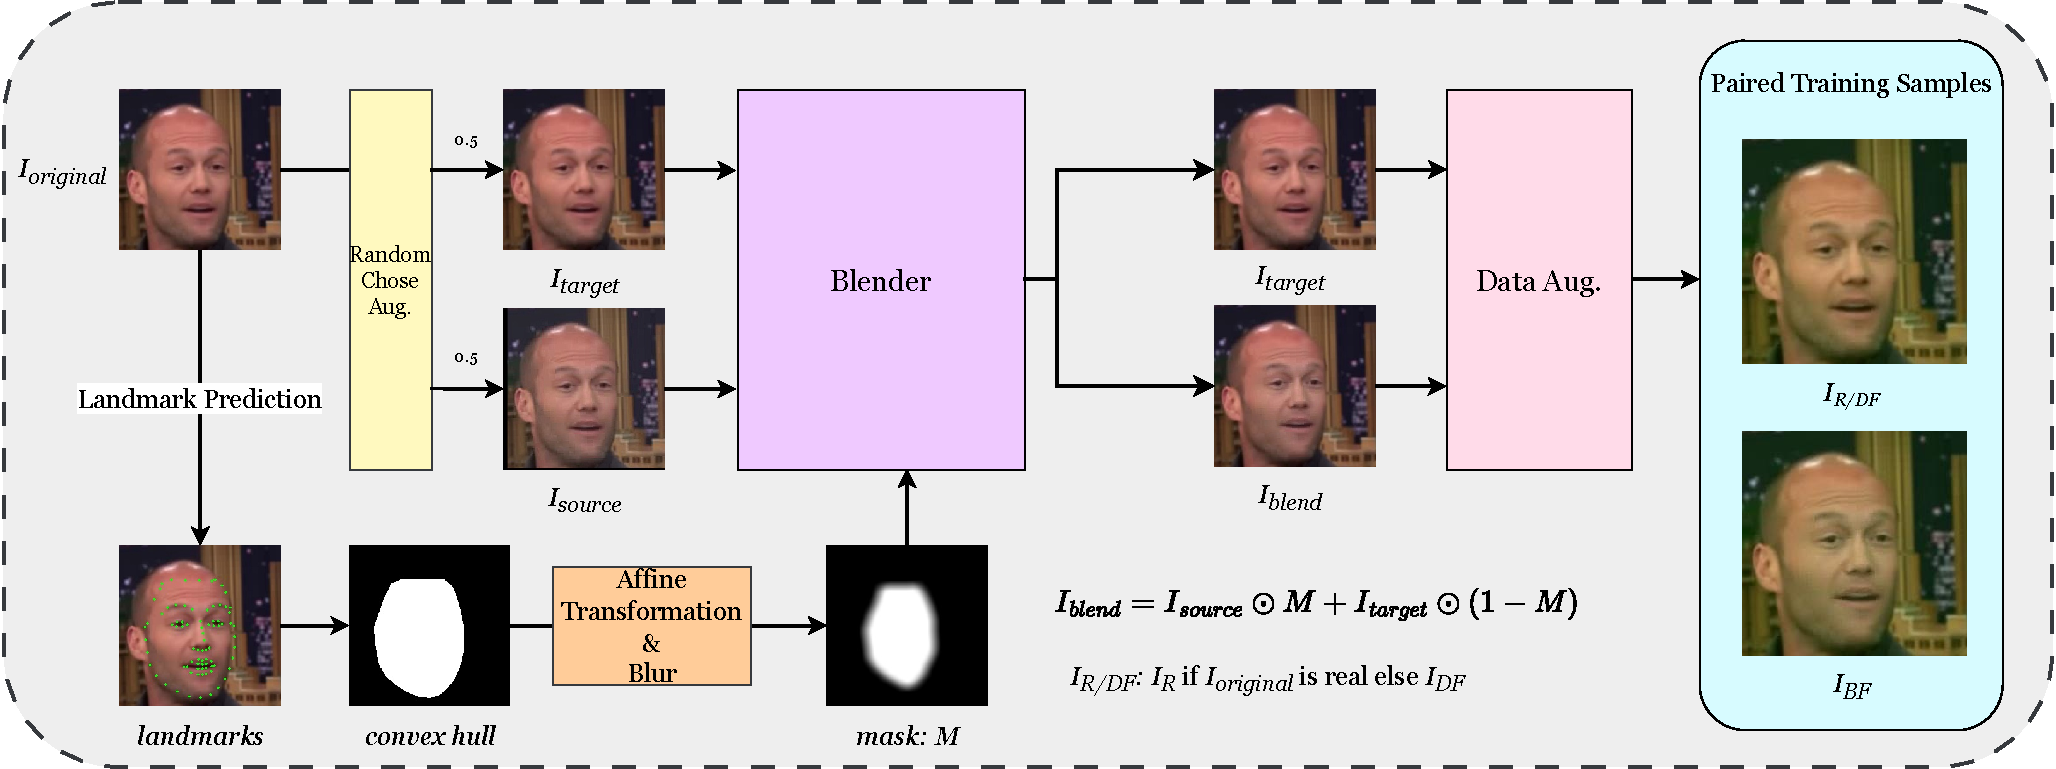
\includegraphics[width=1.0\linewidth]{images/Fig4.pdf}
\caption{Workflow of the PTSG module. Given an original image $I_{original}$, the module generates a paired training sample consisting of an augmented real or deepfake image $I_{R/DF}$ and an augmented self-blended fake image $I_{BF}$.} 
\label{Fig4}
\end{figure*}

\begin{figure*}[htb]
\centering
\includegraphics[width=1.0\linewidth]{images/Fig5.pdf}
\caption{Examples of training samples generated by the PTSG module. The top row illustrates the transformation from a real image to a self-blended fake image, while the bottom row shows the transformation from a deepfake image to a self-blended fake image.} 
\label{Fig5}
\end{figure*}

Before training, the input image $I_{original}$ is processed by the Paired Training Samples Generator (PTSG) to produce a labeled sample pair $((I_{R/DF},I_{BF}),t)$. This module integrates data augmentation with a self-blending transformation method \cite{18} to generate two variants: an augmented image $I_{R/DF}$ and a self-blended fake image $I_{BF}$. If $I_{original}$ is a real image, the label $t$ is set to 0; otherwise, it is set to 1. Fig \ref{Fig4} illustrates the workflow of the PTSG module.

The blending mask $M$ is derived from facial landmarks predicted by a facial keypoint detector \cite{32}, which identifies 81 keypoints to construct a convex hull. This hull is subsequently refined through affine transformations and Gaussian blur, resulting in the final mask $M$. The image $I_{original}$ is divided into two versions: $I_{source}$ and $I_{target}$, where the latter serves as the background and the former provides foreground content. One of them is randomly selected for data augmentation.

The augmentation process introduces variability in several aspects. With a $30\%$ probability, the RGB channels are shifted by $\pm20$ units. Hue, saturation and value are each adjusted by a random value in the range $[-0.3,0.3]$, while brightness and contrast are independently perturbed within $[-0.1,0.1]$. To simulate diverse image qualities, the image is randomly subjected to either $2\times$ or $4\times$ downsampling or sharpening. The blended image $I_{blend}$ is computed using the Equation (\ref{eq1}):
\begin{equation} \label{eq1}
I_{blend}=I_{source} \odot M+I_{target} \odot (1-M).
\end{equation}

After blending, both $I_{target}$ and $I_{blend}$ undergo a second round of augmentation to enhance robustness to variations in illumination, color, and compression artifacts. This includes an additional $30\%$ chance of applying RGB bias within range of $[-20,20]$, further jittering of hue, saturation and value within $[-0.3,0.3]$, as well as variations in brightness and contrast also within $[-0.3,0.3]$. Moreover, JPEG compression is optionally applied with a probability of $50\%$, using a randomly selected quality level between $40$ and $100$.

Fig \ref{Fig5} shows examples of training sample pairs produced by the PTSG module. For real images $I_R$, the paired self-blended image $I_{BF}$ forms a negative pair labeled $t=0$, indicating a low similarity. Conversely, for deepfake images $I_{DF}$, the paired $I_{BF}$ constitutes a positive pair labeled $t=1$, suggesting higher semantic similarity. This labeling system is fully compatible with the traditional "0 for real, 1 for fake" supervised learning paradigm \cite{33}, allowing seamless integration into existing deepfake detection models without relabeling the original dataset.

\subsection{Model Architecture} \label{ma}

\begin{figure*}[htb]
\centering
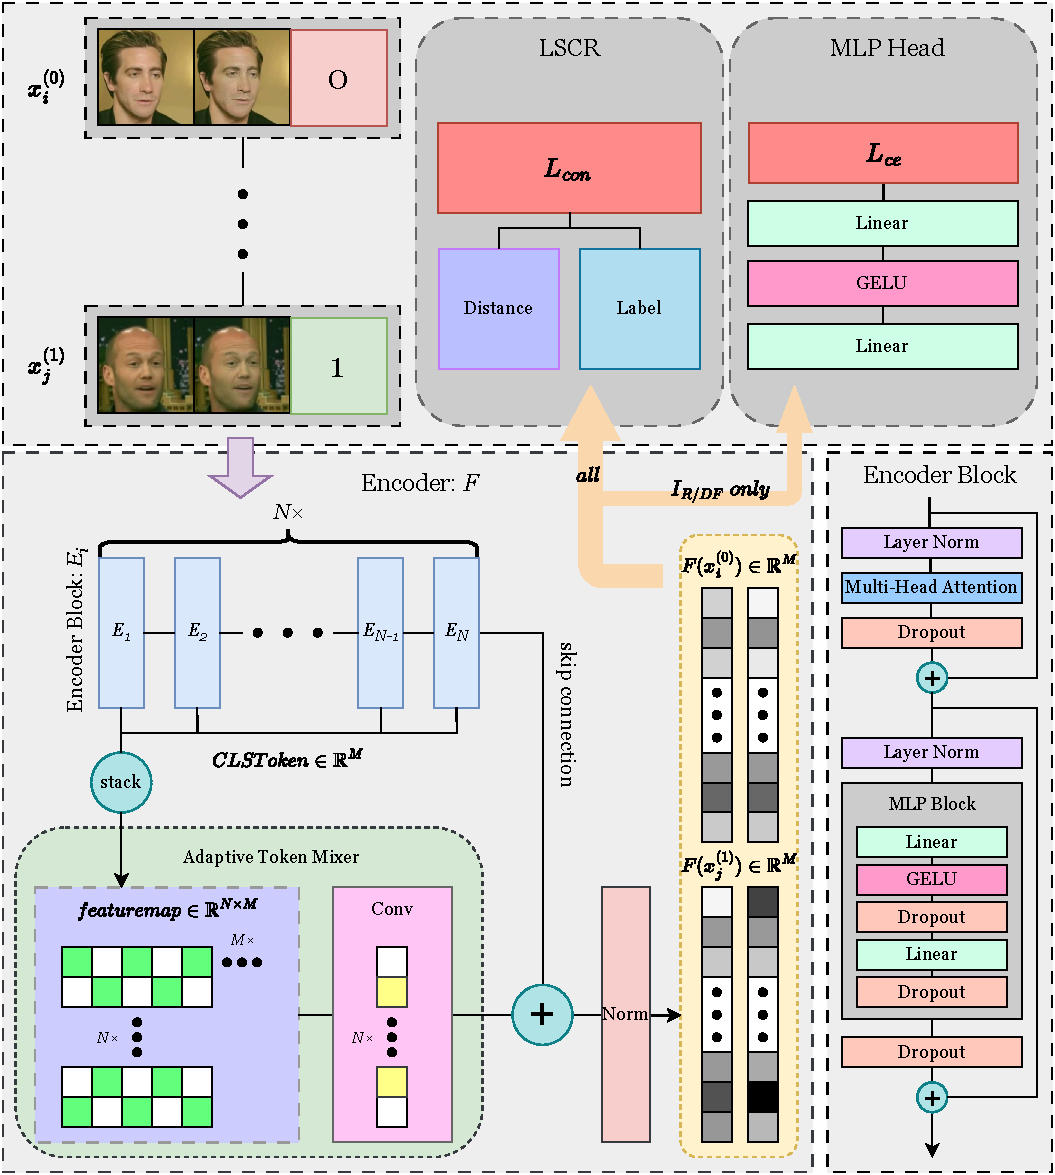
\includegraphics[width=0.75\linewidth]{images/Fig6.pdf}
\caption{Detailed architecture of the proposed network. The model receives paired inputs generated by the PTSG module. Features are extracted via the encoder $F$, and the resulting representations are processed by the LSCR module to compute the contrastive loss $L_{con}$. The feature vector corresponding to $I_{R/DF}$ is further passed through the MLP Head to produce the prediction logits and compute the cross-entropy loss $L_{ce}$ for the final classification decision.} 
\label{Fig6}
\end{figure*}

We propose a model for paired sample feature extraction and loss computation, with its detailed architecture illustrated in Fig \ref{Fig6}. The core components of the network include a feature encoder (Encoder), a Latent Space Contrastive Regularization (LSCR) module, and a classification head (MLP Head).

Our model adopts the small variant of Dinov2 \cite{31} as the backbone, which is based on the Vision Transformer (ViT-S/14) architecture. It comprises 12 Transformer blocks $(N=12)$, as shown in the Encoder Block of Figure 6. Each input image is split into 256 patch tokens, with an additional CLSToken appended for global representation. Each token is embedded into a 384-dimensional vector $(M=384)$. The multi-head self-attention mechanism includes 6 attention heads. In the MLP Block, the first linear layer expands the token dimension from 384 to 1536, and the second layer reduces it back to 384. The final output is a 384-dimensional feature vector representing the input.

During training, the network receives paired inputs $x_i^{(t)}$ generated by the PTSG module. Each training sample is passed through the N-layer encoder stack $E_i$ to extract hierarchical features, where the CLSToken from each layer is collected as a representation of that layer.

To effectively aggregate information across layers, we design an Adaptive Token Mixer (ATM), which employs a 1D convolution to compute a dynamic weighted sum of all CLSToken across the Transformer layers. The feature aggregation is computed as Equation (\ref{eq2}):
\begin{equation} \label{eq2}
f_{ATM}=\sum_{i=1}^N w_i \cdot CLS^i,
\end{equation}
where $w_i$ is the learnable weight from the 1D convolution kernel corresponding to layer $i$, and $CLS^i$ is the CLSToken output from the $i$-th encoder block.

The final feature representation \( F(x_i^{(t)}) \) is obtained by adding \( f_{ATM} \) to the CLSToken from the last encoder block \( E_N \), followed by layer normalization. This fused feature vector contains representations for both sample types: features from real or deepfake images, denoted as \( F(I_{R/DF}) \), and features from self-blended fake images, denoted as \( F(I_{BF}) \). Both types of features are then passed into the LSCR module, where the contrastive loss \( L_{con} \) is computed (see Section \ref{tp} for details).

In the classification stage, only $F(I_{R/DF})$ is passed into the MLP Head, which performs the final binary classification task and computes the cross-entropy loss $L_{ce}$.

\subsection{Training Pipeline} \label{tp}

Unlike naive hybrid training strategies that directly treat blendfake samples as classification inputs, our approach uses these samples as implicit supervision signals for contrastive learning. Specifically, we pair both real and deepfake samples with their corresponding self-blended versions, and introduce the blendfake feature information through the LSCR module.

All self-blended samples are uniformly assigned the forged label to impose dual constraints on the encoder. Specifically, the LSCR module enforces a clear separation in the embedding space between real images and their self-blended counterparts, while simultaneously encouraging the representations of deepfake images to be close to those of their corresponding self-blended versions in the latent space.

This innovative use of self-blended samples as implicit data augmentation allows the model to dynamically construct a diverse set of forgeries with abnormal statistical characteristics, without relying on external samples. By applying bi-directional blending to both real and deepfake samples, the model generates more challenging training signals while preserving the native semantics of deepfakes.

Finally, the model jointly optimizes cross-entropy loss $L_{ce}$ and contrastive loss $L_{con}$, maintaining a clean binary classification framework while regulating feature distribution in latent space. This enhances generalization and prevents the feature space collapse that often occurs in naive hybrid training.

For binary classification, the MLP Head computes the cross-entropy loss $L_{ce}$. Given a batch of $n$ images denoted as $X=\{x_0,x_1,\dots,x_i,\dots,x_{n-1}\},$ where each $x_i$ represents an individual image sample in the batch. Correspondingly, their labels are given by $T=\{t_0,t_1,\dots,t_i,\dots,t_{n-1}\}$, where each $t_i$ denotes the label associated with the image $x_i$. Specifically, $t_i=0$ indicates a real image, and $t_i=1$ indicates a fake image. Let $\hat{t}_i \in [0,1]$ denote the model's prediction for image $x_i$. The classification loss is defined as Equation (\ref{eq3}):
\begin{equation} \label{eq3}
L_{ce}=-\frac{1}{n} \sum_{i=0}^{n-1}(t_ilog⁡\hat{t_i}+(1-t_i)log⁡(1-\hat{t_i})).
\end{equation}

To optimize latent space distribution, the LSCR module employs supervised contrastive learning to pull together the embeddings of similar pairs and push apart dissimilar ones. Let $S= \{s_0,s_1,\dots,s_i,\dots,s_{n-1}\}$ be the set of self-blended images corresponding to the original inputs. When $t_i=0$, the pair $(x_i,s_i)$ is treated as dissimilar (i.e., real and blendfake); when $t_i=1$, the pair is similar (i.e., deepfake and blendfake). Let $F(\cdot)$ denote the encoder, and $\alpha$ a contrastive margin. The contrastive loss is defined as Equation (\ref{eq4}):
\begin{equation} \label{eq4}
L_{con}=\frac{1}{n}\sum_{i=0}^{n-1}(t_i\|F(x_i)-F(s_i)\|_2+(1-t_i)max(0,\alpha-\|F(x_i)-F(s_i)\|_2)).
\end{equation}

This formulation enforces two contrasting behaviors depending on the label \( t_i \). When \( t_i = 0 \), the objective is to maximize the distance \( \|F(x_i) - F(s_i)\|_2 \), thereby pushing the real image and its self-blended counterpart apart in the feature space. In contrast, when \( t_i = 1 \), the goal is to minimize this distance, encouraging the deepfake image and its self-blended version to lie close together in the latent space.

The overall loss is a weighted sum of classification and contrastive losses, overall loss is defined as Equation (\ref{eq5}):
\begin{equation} \label{eq5}
L_{overall}=L_{ce}+\beta L_{con},
\end{equation}
where $\beta$ is a hyperparameter controlling the strength of contrastive regularization.

The model is trained using the Adam optimizer, with a step decay learning rate schedule. The learning rate is reduced by a factor of $\gamma$ after each step. In the contrastive loss, the margin $\alpha$ is set to 1.0, and the contrastive loss weight $\beta$ is set to 0.5. All remaining training hyperparameters are detailed in Table \ref{tab1}. Algorithm 1 presents the pseudocode of our proposed method, which leverages the GHT framework to enhance the robustness of deepfake detection.

\begin{table}
    \centering
    \begin{tabular}{cc}\toprule
         Hyperparameter& Value
\\\midrule
         batchsize& $32$\\
         learning rate& $10^{-5}$\\
         epochs& $20$\\
         step& $3$\\
         gamma& $0.4$\\ \bottomrule
    \end{tabular}
    \caption{Training hyperparameters used in our experiments.}
    \label{tab1}
\end{table}

\begin{algorithm}[htb]
\renewcommand{\algorithmicrequire}{\textbf{Input:}}
\renewcommand{\algorithmicensure}{\textbf{Initialization:}}
\caption{Generalizable Hybrid Training for Robust Deepfake Detection}
\label{alg:hybrid_training}
\begin{algorithmic}[1]
\REQUIRE ~~\\
    Image $I_{\text{original}} \in \mathbb{R}^{H \times W \times 3}$ with label $t$; \\
    Facial landmarks $L \in \mathbb{R}^{81 \times 2}$
\ENSURE ~~\\
    Trained encoder parameters $\theta_f$, MLP head parameters $\theta_h$ \\
    Initialize encoder $F$ with parameters $\theta_f$ using pretrained Dinov2; \\
    Initialize MLP head $h$ with parameters $\theta_h$ randomly; \\
    Generate training pairs using a facial blend function
\STATE \textbf{Training stage:}
\FOR{each $((I_{\text{R/DF}}, I_{\text{BF}}), t)$ in dataloader}
    \STATE Extract features:
    \STATE \quad $f_{\text{R/DF}} = F(I_{\text{R/DF}} \mid \theta_f)$
    \STATE \quad $f_{\text{BF}} = F(I_{\text{BF}} \mid \theta_f)$
    \STATE Compute distance $D$:
    \STATE \quad $D = \text{distance}(f_{\text{R/DF}}, f_{\text{BF}})$
    \STATE Compute contrastive loss:
    \STATE \quad $L_{\text{con}} = tD + (1 - t)\max(0, \alpha - D)$
    \STATE Predict label and compute cross-entropy loss:
    \STATE \quad $\hat{t} = h(f_{\text{R/DF}} \mid \theta_h)$
    \STATE \quad $L_{\text{ce}} = tlog⁡\hat{t}+(1-t)log⁡(1-\hat{t})$
    \STATE Combine losses and update parameters:
    \STATE \quad $L_{\text{overall}} = L_{\text{ce}} + \beta L_{\text{con}}$
    \STATE \quad Update $\theta_f$, $\theta_h$ via backpropagation
\ENDFOR
\RETURN $\theta_f$, $\theta_h$
\end{algorithmic}
\end{algorithm}

\section{Experiments} \label{e}

\subsection{Experimental Setup}

We implemented our model on the DeepfakeBench platform \cite{33}, which provides a unified data management system to ensure consistent input across all detection models. In addition, the platform defines standardized evaluation metrics and protocols to promote transparency and reproducibility in performance comparisons. All training and testing were conducted on a workstation equipped with an NVIDIA RTX 4090 GPU (24 GB VRAM).

An overview of all datasets used in our experiments is provided in Table \ref{tab2}. To ensure a comprehensive and fair evaluation of the model's generalization capability, we adopt widely used deepfake datasets for training. Specifically, we use the FaceForensics++ (FF++) dataset \cite{25}, which includes four forgery methods: Deepfakes (DF) \cite{34}, Face2Face (F2F) \cite{35}, FaceSwap (FS) \cite{36}, and NeuralTextures (NT) \cite{37}. In all experiments, we use the low-quality version (FF++ LQ) as the training set. The real images used to generate self-blended forgeries also originate from the FF++ (LQ) dataset. Unless otherwise specified, references to FF++ in the remainder of the paper refer to the LQ version by default.

To evaluate cross-domain generalization, we utilize four challenging and diverse benchmark datasets: Celeb-DFv1\cite{19}, Celeb-DFv2\cite{19}, Deepfake Detection Challenge Preview (DFDCP)\cite{20}, and Deepfake Detection Challenge (DFDC)\cite{21}. These datasets encompass a broad spectrum of facial identities, recording environments, and forgery techniques. Their inherent variability makes them particularly well-suited for rigorously assessing the robustness and generalization capabilities of deepfake detection models.

To ensure fair comparisons, our model and all baseline methods follow the standardized settings defined by DeepfakeBench \cite{33}. During the data preprocessing stage, we randomly sample 32 frames from each video. DLIB \cite{38} is used for face detection, cropping, and alignment. The aligned face images are then resized to $256\times256$ pixels, and used as input for both training and testing. In the training pipeline, to maintain parameter parity with baseline models, we adopt the Dinov2-small variant as our backbone network.

\begin{table*}[]\rmfamily
    \centering
    \caption{Overview of datasets used in experiments. The table reports the number of real videos, fake videos, total videos, number of subjects, and the number of forgery methods for each dataset.}
    \label{tab2}
\begin{tabular}{cccccc}
\toprule
Dataset& Real Videos& Fake Videos&     Total Videos& Total Subjects&Synthesis Methods\\\midrule
                       FaceForensics++&                         1000& 4000& 5000& N/A& 4
\\ 
Celeb-DFv1& 408& 795& 1203& N/A& 1
\\
                       Celeb-DFv2& 590& 5639&                       6229& 59& 1
\\
DFDCP& 1131& 4119& 5250& 66& 2
\\
                       DFDC& 23654& 104500&                       128154& 960& 8
\\ \bottomrule
\end{tabular}
\end{table*}

\subsection{Evaluation Metrics}

$AUC$ (Area Under the Curve) is the most widely used evaluation metric for assessing the performance of detection models \cite{33}. In this study, we primarily adopt $AUC$ to evaluate model performance across datasets. $AUC$ refers to the area under the ROC (Receiver Operating Characteristic) curve, which is constructed by comparing the $TPR$ (True Positive Rate) and the $FPR$ (False Positive Rate) at various classification thresholds. It provides a holistic view of the classifier's ability to distinguish between real and fake samples.

To construct the ROC curve and compute the $AUC$, classification thresholds are first defined to separate positive and negative classes. For each threshold, $TPR$ and $FPR$ are computed using Equations (\ref{eq6}) and Equation (\ref{eq7}), respectively:
\begin{equation} \label{eq6}
TPR=\frac{TP}{TP+FN},
\end{equation}
\begin{equation} \label{eq7}
FPR=\frac{FP}{FP+TN},
\end{equation}
where $TP$ (True Positive)  denotes the number of correctly predicted positive samples, $TN$ (True Negative) refers to the number of correctly predicted negative samples. $FP$ (False Positive) is the number of negative samples that are incorrectly predicted as positive, while $FN$ (False Negative) represents the number of positive samples that are incorrectly predicted as negative. By plotting $TPR$ against $FPR$ across all thresholds, the ROC curve is formed, and the area under this curve is calculated to reflect the model's performance across all operating points.

In Section 4.2.2 (Comprehensive Evaluation), we additionally report $ACC$ (Accuracy), $EER$ (Equal Error Rate) and $AP$ (Average Precision) as supplementary metrics. $ACC$ measures the overall correctness of predictions, defined in  Equation (\ref{eq8}):
\begin{equation} \label{eq8}
ACC=\frac{TP+TN}{TP+TN+FP+FN}.
\end{equation}

$EER$ is the error rate at the threshold where $FPR$ equals the $FNR$ (False Negative Rate), which is defined in Equation (\ref{eq9}):
\begin{equation} \label{eq9}
FNR=\frac{FP}{TP+FN}.
\end{equation}
The threshold at which $FPR$ and $FNR$ are closest (or intersect) is used to determine the $EER$.

$AP$ (Average Precision) quantifies the area under the Precision-Recall (PR) curve, reflecting the average performance of the model at all recall levels. It is calculated as Equation (\ref{eq10}):
\begin{equation} \label{eq10}
AP=\sum_n(R_N-R_{n-1})P_n,
\end{equation}
where $P_n$ and $R_n$ denote the precision and recall at the $n$-th sample, defined respectively in Equation (\ref{eq11}) and Equation (\ref{eq12}):
\begin{equation} \label{eq11}
Precision=\frac{TP}{TP+FP},
\end{equation}
\begin{equation} \label{eq12}
Recall=\frac{TP}{TP+FN}.
\end{equation}

By computing multiple $(Precision, Recall)$ pairs across different thresholds and integrating the resulting curve, $AP$ provides a summary of performance across varying decision boundaries.

\subsection{Baseline Methods}

To comprehensively evaluate the generalization ability of our proposed method, we compare it against several representative and state-of-the-art baseline models in the field of deepfake detection \cite{10,18,25,28}. These baselines cover a range of architectural designs and training strategies, including traditional CNN-based models, blendfake based approaches, RGB–frequency domain fusion methods, and feature disentanglement methods. A brief overview of each method is provided below:

\begin{itemize}
    \item \textbf{Xception} \cite{25}: Xception is an advanced visual recognition model based on depthwise separable convolutions. Due to its outstanding performance in deepfake detection, it has been selected as the baseline model in the FaceForensics++ (FF++) dataset. Moreover, Xception has been widely adopted in numerous related studies as a strong benchmark for performance comparison.
    \item \textbf{SBI} \cite{18}: SBI is a state-of-the-art forgery detection model based on self-blended image training. It synthesizes subtle and hard-to-detect fake samples by blending real images using learnable masks, thereby enhancing the model's sensitivity to forgery artifacts and improving detection performance.
    \item \textbf{LRL} \cite{28}: LRL proposes a local relational learning approach for deepfake detection. The core idea is to model relationships between local regions to precisely capture manipulation traces. It further integrates multi-scale RGB and frequency domain features to improve detection accuracy and generalization across various forgery types.
    \item \textbf{UCF} \cite{10}: UCF introduces a disentangled feature learning framework that decomposes image features into content, forgery-specific, and forgery-generic components. Only the forgery-generic features are used for classification, effectively reducing the model's dependence on specific manipulation techniques. UCF achieves state-of-the-art performance on the DeepfakeBench platform.
\end{itemize}

\subsection{Comprehensive Generalization Evaluation}

\begin{table*}[htb]
\rmfamily
\centering
\caption{Cross-dataset generalization comparison of multiple models. The table reports AUC, ACC, EER, and AP on four benchmark datasets: Celeb-DFv1, Celeb-DFv2, DFDC, and DFDCP. The best result for each dataset and metric is highlighted in bold. Avg. denotes the average score across all benchmark datasets.}
\label{tab3}
\begin{tabular}{>{\centering\arraybackslash}m{2.0cm}>{\centering\arraybackslash}m{1.5cm}|*{5}{>{\centering\arraybackslash}m{2.0cm}}}
\toprule
\multirow{2}{*}{\textbf{Method}} & \multirow{2}{*}{\textbf{Metric}} & \multicolumn{5}{c}{\textbf{Test set (\%)}} \\
\cmidrule(lr){3-7}
& & \textbf{Celeb-DFv1} & \textbf{Celeb-DFv2} & \textbf{DFDCP} & \textbf{DFDC} & \textbf{Avg.} \\
\midrule

\multirow{4}{*}{Xception \cite{25}} 
& AUC & 72.62 & 72.77 & 70.06 & 72.95 & 72.10 \\
& ACC & 66.14 & 70.24 & 69.92 & 66.18 & 68.12 \\
& EER & 32.50 & 33.52 & 35.18 & 33.99 & 33.80 \\
& AP  & 81.31 & 82.20 & 78.23 & 75.15 & 79.22 \\

\midrule
\multirow{4}{*}{LRL \cite{28}} 
& AUC & 79.44 & 75.77 & 69.11 & 67.66 & 73.00 \\
& ACC & 72.61 & 71.41 & 65.55 & 62.24 & 67.95 \\
& EER & 28.35 & 31.87 & 36.23 & 37.75 & 33.55 \\
& AP  & 87.19 & 84.64 & 79.75 & 69.64 & 80.31 \\

\midrule
\multirow{4}{*}{SBI \cite{18}} 
& AUC & 79.51 & 78.22 & 70.75 & 61.31 & 72.45 \\
& ACC & 58.10 & 47.27 & 51.39 & 52.55 & 52.33 \\
& EER & 28.76 & 28.63 & 33.71 & 42.30 & 33.35 \\
& AP  & 86.72 & 86.62 & 81.83 & 65.25 & 80.11 \\

\midrule
\multirow{4}{*}{UCF \cite{10}} 
& AUC & 81.11 & 77.16 & 69.27 & 73.15 & 75.17 \\
& ACC & 72.74 & 64.91 & 59.53 & 65.76 & 65.74 \\
& EER & 27.10 & 30.32 & 35.76 & 33.61 & 31.70 \\
& AP  & 88.73 & 86.06 & 79.18 & 75.07 & 82.26 \\

\midrule
\multirow{4}{*}{\textbf{Ours}} 
& AUC & \textbf{84.73} & \textbf{84.95} & \textbf{75.95} & \textbf{75.70} & \textbf{80.33} \\
& ACC & \textbf{76.63} & \textbf{78.69} & \textbf{71.11} & \textbf{68.39} & \textbf{73.71} \\
& EER & \textbf{22.11} & \textbf{23.42} & \textbf{31.72} & \textbf{31.77} & \textbf{27.26} \\
& AP  & \textbf{89.78} & \textbf{90.38} & \textbf{85.17} & \textbf{77.23} & \textbf{85.64} \\

\bottomrule
\end{tabular}
\end{table*}

To thoroughly evaluate and compare the cross-dataset generalization ability of different models, we conduct benchmarking on four widely-used datasets: Celeb-DFv1, Celeb-DFv2, DFDC, and DFDCP. We compare our model against several state-of-the-art approaches based on different methodologies. The results are summarized in Table \ref{tab3}.

All baseline models are trained using FF++ dataset on the DeepfakeBench \cite{33} platform, ensuring consistency in experimental settings. In addition to the primary metric AUC (Area Under the ROC Curve), we report three complementary metrics: Accuracy (ACC), Equal Error Rate (EER), and Average Precision (AP) to provide a more comprehensive assessment of each model's generalization performance.

As shown in Table \ref{tab3}, our proposed method consistently outperforms all compared baselines across all four benchmark datasets and evaluation metrics. Specifically, it achieves the highest AUC scores on Celeb-DFv1 (84.73\%), Celeb-DFv2 (84.95\%), DFDCP (75.95\%), and DFDC (75.70\%), leading to the best average AUC of 80.33\%. In terms of classification accuracy (ACC), our model also shows substantial improvements, with an average ACC of 73.71\%, outperforming the second-best method by a margin of over 5\%. Furthermore, our approach achieves the lowest Equal Error Rate (EER) of 27.26\%, indicating a better trade-off between false positives and false negatives.

The improvements are particularly significant on challenging datasets like DFDC and DFDCP, where other models struggle to generalize. For instance, compared to the SBI method, our model improves AUC on DFDC by over 14\%, and increases AP from 65.25\% to 77.23\%. These results demonstrate the strong generalization ability of our method across diverse forgery types and domains, validating the effectiveness of the proposed training strategy and feature representation design.

\subsection{Ablation Study}

\begin{table*}[htb]\rmfamily
    \centering
    \caption{AUC (\%) performance of the model trained with different latent space distance metrics across FF++, Celeb-DFv1, Celeb-DFv2, DFDCP, and DFDC datasets.}
    \label{tab4}
\begin{tabular}{ccccccc}\toprule                    													            														

Metric& \multicolumn{1}{c}{FF++} & Celeb-DFv1&                         Celeb-DFv2& DFDCP&                         DFDC& Average
\\\midrule Cosine& \multicolumn{1}{c}{96.65 }                        & \multicolumn{1}{c}{81.36 } & \multicolumn{1}{c}{82.64 } & \multicolumn{1}{c}{77.18 } & \multicolumn{1}{c}{76.28 } & \multicolumn{1}{c}{82.82 
}  \\ 
Euclidean& \multicolumn{1}{c}{96.05 }                        & \multicolumn{1}{c}{84.73 }    & \multicolumn{1}{c}{84.59 }     & \multicolumn{1}{c}{75.95 }    & \multicolumn{1}{c}{75.70 }     & \multicolumn{1}{c}{83.40 
}         \\ \bottomrule 
\end{tabular}
\end{table*}

\begin{table}[htb]\rmfamily
    \centering
    \caption{A comprehensive comparison between our proposed model and the state-of-the-art BlendFake training-based model SBI \cite{18} under five different training configurations. FF-ALL denotes training on all manipulation methods from the FaceForensics++ dataset, while FF-w/o-F2F, FF-w/o-DF, FF-w/o-FS, and FF-w/o-NT represent training without Face2Face, Deepfakes, FaceSwap, and NeuralTextures, respectively. This evaluation highlights each model's robustness and generalization performance under varying supervision conditions.}
    \label{tab5}
    \begin{tabular}{llcc}
        \toprule
        \multicolumn{2}{c}{\multirow{2}{*}{\textbf{Settings}}} & \multicolumn{2}{c}{Method}\\
 \cmidrule(lr){3-4}& & \textbf{SBI}&\textbf{Ours} \\
        \cmidrule(lr){1-2} \cmidrule(lr){3-4}
        
        \multirow{4}{*}{FF-ALL} 
        & Celeb-DFv1  & 79.51 & 84.73 ($\uparrow \,$ 5.22) \\
        & Celeb-DFv2  & 78.22 & 84.59 ($\uparrow \,$ 6.37) \\
        & DFDCP       & 70.75 & 75.70 ($\uparrow \,$ 4.95) \\
        & DFDC        & 61.31 & 75.95 ($\uparrow$14.64) \\
        \cmidrule(lr){2-4}

        \multirow{4}{*}{FF-w/o-F2F} 
        & Celeb-DFv1  & 64.91 & 76.38 ($\uparrow$11.47) \\
        & Celeb-DFv2  & 74.57 & 83.99 ($\uparrow \,$ 9.42) \\
        & DFDCP       & 76.23 & 76.86 ($\uparrow \,$ 0.63) \\
        & DFDC        & 66.18 & 77.62 ($\uparrow$11.44) \\
        \cmidrule(lr){2-4}

        \multirow{4}{*}{FF-w/o-DF} 
        & Celeb-DFv1  & 77.53 & 74.58 ($\downarrow \,$ 2.95) \\
        & Celeb-DFv2  & 76.14 & 75.23 ($\downarrow \,$ 0.91) \\
        & DFDCP       & 73.15 & 66.22 ($\downarrow \,$ 6.93) \\
        & DFDC        & 63.60 & 67.61 ($\uparrow \,$ 4.01) \\
        \cmidrule(lr){2-4}

        \multirow{4}{*}{FF-w/o-FS} 
        & Celeb-DFv1  & 72.27 & 78.99 ($\uparrow \,$ 6.72) \\
        & Celeb-DFv2  & 75.25 & 78.77 ($\uparrow \,$ 3.52) \\
        & DFDCP       & 74.38 & 72.09 ($\downarrow \,$ 2.29) \\
        & DFDC        & 64.63 & 71.48 ($\uparrow \,$ 6.85) \\
        \cmidrule(lr){2-4}

        \multirow{4}{*}{FF-w/o-NT} 
        & Celeb-DFv1  & 77.45 & 85.98 ($\uparrow \,$ 8.53) \\
        & Celeb-DFv2  & 72.48 & 80.90 ($\uparrow \,$ 8.42) \\
        & DFDCP       & 67.64 & 78.35 ($\uparrow$10.71) \\
        & DFDC        & 62.36 & 74.98 ($\uparrow$12.62) \\
        \midrule
        \multicolumn{2}{c}{\textbf{Average}} & \textbf{71.43} & \textbf{77.05 ($\uparrow \,$ 5.62)} \\
        \bottomrule
    \end{tabular}
\end{table}

\begin{table*}[htb]\rmfamily
    \centering
    \caption{AUC (\%) comparison of different training strategies on four generalization benchmarks: Celeb-DFv1, Celeb-DFv2, DFDCP, and DFDC. DOT: Deepfake-Only Training; BOT: Blendfake-Only Training; NHT: Naive Hybrid Training; Ours: Our method with latent space contrastive regularization.}
    \label{tab6}
\begin{tabular}{cccccc}\toprule                    													            														

Method& \multicolumn{1}{c}{Celeb-DFv1} & Celeb-DFv2&                         DFDCP& DFDC&                         Average
\\\midrule DOT& \multicolumn{1}{c}{74.88 }                        & \multicolumn{1}{c}{75.83 } & \multicolumn{1}{c}{73.46 } & \multicolumn{1}{c}{68.09 } & \multicolumn{1}{c}{73.07 
}   \\ 
BOT& \multicolumn{1}{c}{78.61 }                        & \multicolumn{1}{c}{81.02 }    & \multicolumn{1}{c}{73.25 }     & \multicolumn{1}{c}{75.90 }    & \multicolumn{1}{c}{77.20 
}              \\ 
 NHT& 76.38 & 78.64 & 72.88 & 73.76 &75.42 
\\
 Ours& 84.73 & 84.59 & 75.95 & 75.70 &80.24 
\\ \bottomrule 
\end{tabular}
\end{table*}

We analyze the effect of distance metrics within the LSCR module by comparing Euclidean distance and cosine similarity, as reported in Table \ref{tab4}. While cosine similarity yields marginally higher performance on intra-domain (FF++) evaluation, Euclidean distance demonstrates superior generalization across multiple benchmark datasets. Consequently, we select Euclidean distance as the default choice for all following experiments.

The stability of the model under different combinations of training data is evaluated using a "leave-one-out" training approach on the FF++ dataset. Table~\ref{tab5} compares the AUC performance of the SBI model, trained solely on blendfake data, and our model under this setting. As shown in the table, except for the case where FF-DF is excluded, which significantly impacts the generalization performance of our model, our method consistently outperforms the SBI model in all other settings. The average AUC improvement over SBI across all settings is 5.62\%, indicating that our approach effectively leverages both blendfake and deepfake forgery information to enhance the generalization capability of the detection model.

To investigate how different training strategies affect cross-domain generalization in deepfake detection, we design four distinct experimental configurations:

\begin{enumerate}
    \item \textbf{Deepfake-Only Training (DOT):} The Dinov2-small backbone is fine-tuned exclusively on FF++ deepfake samples. This setup omits any additional training signals such as blended forgeries or regularization.
    
    \item \textbf{Blendfake-Only Training (BOT):} The model is trained solely on self-blended forgeries created within the FF++ domain. These samples, while synthetically generated, often present more localized and nuanced manipulations, making them particularly challenging for detection.
    
    \item \textbf{Naive Hybrid Training (NHT):} This configuration combines FF++ deepfake and blendfake data in a straightforward joint training setup, without any latent space regularization or adaptive token mix mechanisms.
    
    \item \textbf{Generalizable Hybrid Training (Ours):} Our proposed strategy incorporates siamese networks with a latent space contrastive regularization module and an adaptive token mixer, enabling more effective feature integration from both deepfake and blendfake samples.
\end{enumerate}

As shown in Table \ref{tab6}, the DOT approach, despite its simplicity, achieves a surprisingly competitive average AUC of \textbf{73.07\%}, outperforming several existing methods. This outcome highlights the strength of the pretrained Dinov2 features in transfer learning for deepfake detection. BOT further improves generalization performance by leveraging the difficulty and diversity of self-blended forgeries, which serve as effective hard examples. In contrast, the NHT strategy results in a performance drop, indicating that naive data-level fusion without considering latent space alignment can introduce representational conflicts and degrade model robustness. Our contrastive regularization approach overcomes this limitation by structurally organizing the latent space, allowing the model to fully exploit complementary information from both data sources. This leads to superior performance across all benchmarks, confirming the effectiveness of our design in enhancing cross-domain generalization.


\subsection{Visualization Analysis}

\begin{figure*}[htb]
\centering
\includegraphics[width=1\linewidth]{images/Fig7.pdf}
\caption{t-SNE visualization of the latent features on the FF++ test set. The model was trained on the FF++ training set and evaluated in-domain. We randomly sampled 2,500 real and 2,500 fake samples for feature visualization.} 
\label{Fig7}
\end{figure*}

\begin{figure*}[htb]
\centering
\includegraphics[width=1\linewidth]{images/Fig8.pdf}
\caption{t-SNE visualization of latent features under cross-domain generalization. The model was trained on the FF++ training set and tested on four external benchmark datasets. For each dataset, 2,500 real and 2,500 fake samples were randomly selected for visualization.} 
\label{Fig8}
\end{figure*}

To intuitively observe the latent feature distributions learned by the model, we adopt t-SNE \cite{39}, a popular dimensionality reduction technique, to visualize the encoded features in two dimensions.

Figure \ref{Fig7} presents the t-SNE visualization of latent features on the in-domain FF++ test set. As shown in subfigure (a), the features from real and fake samples trained via naive hybrid training are heavily entangled, making it difficult for the classifier to establish a clear decision boundary. In contrast, subfigure (b) shows that our method achieves a better separation of real and fake features in latent space, enabling the model to construct a smoother and more generalizable decision boundary.

To further evaluate the generalization behavior under distribution shifts, we also perform t-SNE visualizations on the model's latent features over four cross-domain datasets. As illustrated in Figure \ref{Fig8}, subfigure (a) shows that the naive hybrid training model suffers from severe feature entanglement in out-of-domain scenarios, showing poor generalization. Meanwhile, subfigure (b) demonstrates that our method maintains well-organized clusters for most samples of the same class. Although some samples exhibit imperfect separation, the inter-class margins in the latent space are more evident, indicating stronger discriminative capability under domain shifts.

\section{Conclusion and Outlook} \label{co}

This study focuses on addressing the generalization problem in deepfake detection, particularly the performance degradation observed during hybrid training with both deepfake and blendfake samples. We identify the root cause of this issue as disorganized latent space representations between deepfake and blendfake. Incorporating blendfake data into training can potentially exacerbate overfitting and impair generalization performance.

To mitigate this problem, we perform transfer learning based on the Dinov2-small backbone and introduce an Adaptive Token Mixing (ATM) mechanism to fully exploit shallow and mid-level features within the network. Our experimental results confirm the backbone's strong performance on deepfake detection tasks.

Moreover, we design a Siamese network architecture that simultaneously utilizes deepfake and blendfake samples to enrich forgery diversity. A key contribution of our method is the introduction of Latent Space Contrastive Regularization (LSCR), which restructures the latent feature space and prevents degradation during hybrid training. Extensive experiments demonstrate that our approach significantly improves model generalization, providing an effective solution to the core challenge in deepfake detection.

Despite the promising results, there remains room for further exploration. From a methodological perspective, our framework can be viewed as a refined extension of existing blendfake training paradigms. In future work, we plan to incorporate incremental learning strategies to improve adaptability. By extending our current architecture into an incremental learning framework, the model can dynamically adapt to and incorporate new types of forgeries, thereby enhancing its robustness against evolving deepfake generation techniques.

\section*{Funding}

This work was supported by the National Natural Science Foundation of China under Grant 62472235.

\section*{CRediT authorship contribution statement}

\textbf{Yapeng Zhi:} Conceptualization, Methodology, Validation, Writing – original draft. \textbf{Xiaolong Xu:} Conceptualization, Funding acquisition, Methodology, Supervision, Writing – review \& editing.

\section*{Declaration of Competing Interest}

The authors declare that they have no known competing financial interests or personal relationships that could have appeared to influence the work reported in this paper.

\section*{Data Availability Statement}

Data and code will be made available on reasonable request.

\section*{Acknowledgements}

We would like to thank the editors and reviewers in advance for their comments and for helping us improve the quality of this paper.

%% If you have bibdatabase file and want bibtex to generate the
%% bibitems, please use
 \bibliographystyle{elsarticle-num} 
 \bibliography{cas-refs}


%% else use the following coding to input the bibitems directly in the
%% TeX file.
 % \bibliographystyle{elsarticle-num} 

% \begin{thebibliography}{00}
%  \bibliography{cas-refs}

% \bibitem{label}
% %% Text of bibliographic item

% % \bibitem{}


% \end{thebibliography}

\end{document}
\endinput
%%
%% End of file `elsarticle-template-num.tex'.
